\documentclass[a4paper,12pt]{article}
%spellchecker
% !TeX spellcheck = de

\usepackage{amssymb} % needed for math
\usepackage{amsmath} % needed for math
\usepackage[utf8]{inputenc} % this is needed for german umlauts
\usepackage[ngerman]{babel} % this is needed for german umlauts
\usepackage[T1]{fontenc}    % this is needed for correct output of umlauts in pdf
\usepackage[margin=2.5cm]{geometry} %layout
\usepackage{booktabs}

% this is needed for forms and links within the text
\usepackage{hyperref}  

% The following is needed in order to make the code compatible
% with both latex/dvips and pdflatex.
\ifx\pdftexversion\undefined
\usepackage[dvips]{graphicx}
\else
\usepackage[pdftex]{graphicx}
\DeclareGraphicsRule{*}{mps}{*}{}
\fi

%%%%%%%%%%%%%%%%%%%%%%%%%%%%%%%%%%%%%%%%%%%%%%%%%%%%%%%%%%%%%%%%%%%%%%
% Variablen                                 						 %
%%%%%%%%%%%%%%%%%%%%%%%%%%%%%%%%%%%%%%%%%%%%%%%%%%%%%%%%%%%%%%%%%%%%%%
\newcommand{\authorName}{Lena Gregor, Dominik Horn}
\newcommand{\auftraggeber}{Lehrstuhl für Datenbanksysteme TUM}
\newcommand{\auftragnehmer}{\authorName}
\newcommand{\projektName}{Wahl und Informationssystem für bayerische Landtagswahlen}
\newcommand{\tags}{\authorName, Lastenheft, TUM, Universität Augsburg, LMU}
\newcommand{\subtitle}{Technische Universität München, Datenbanksysteme WS19/20}

%%%%%%%%%%%%%%%%%%%%%%%%%%%%%%%%%%%%%%%%%%%%%%%%%%%%%%%%%%%%%%%%%%%%%%
% PDF Meta information                                 				       %
%%%%%%%%%%%%%%%%%%%%%%%%%%%%%%%%%%%%%%%%%%%%%%%%%%%%%%%%%%%%%%%%%%%%%%
\hypersetup{
  pdfauthor   = {\authorName},
  pdfkeywords = {\tags},
  pdftitle    = {\projektName~(Lastenheft)}
} 

%%%%%%%%%%%%%%%%%%%%%%%%%%%%%%%%%%%%%%%%%%%%%%%%%%%%%%%%%%%%%%%%%%%%%%
% Custom setup                                                       % 
%%%%%%%%%%%%%%%%%%%%%%%%%%%%%%%%%%%%%%%%%%%%%%%%%%%%%%%%%%%%%%%%%%%%%%
\usepackage{pdfpages}
\usepackage{xcolor,colortbl} 
\definecolor{Blue}{rgb}{0.1,0.2,0.7}
\definecolor{TUMBlue}{HTML}{0065BD}
\definecolor{TUMAccentLightBlue}{HTML}{98C6EA}
\definecolor{TUMLightGray}{HTML}{CCCCC6}
\definecolor{TUMAccentGray}{HTML}{DAD7CB}
\definecolor{lightBlue}{RGB}{157,195,230}


\newcolumntype{b}{>{\columncolor{TUMBlue}}c}
\newcolumntype{a}{>{\columncolor{lightBlue}}c}

\renewcommand{\arraystretch}{1.5}
 
%%%%%%%%%%%%%%%%%%%%%%%%%%%%%%%%%%%%%%%%%%%%%%%%%%%%%%%%%%%%%%%%%%%%%%
% Create a shorter version for tables. DO NOT CHANGE               	 %
%%%%%%%%%%%%%%%%%%%%%%%%%%%%%%%%%%%%%%%%%%%%%%%%%%%%%%%%%%%%%%%%%%%%%%
\newcommand\addrow[2]{\textcolor{black}{#1} &#2\\ \hline}

\newcommand\addheading[2]{\rowcolor{TUMBlue}\textcolor{white}{#1} & \textcolor{white}{#2}\\ \hline}
\newcommand\tabularhead{\begin{tabular}{|a|p{13cm}|}
\hline
}

\newcommand\addmulrow[2]{ \begin{minipage}[t][][t]{2.5cm}#1\end{minipage}% 
   &\begin{minipage}[t][][t]{8cm}
    \begin{enumerate} #2   \end{enumerate}
    \end{minipage}\\ }

\newenvironment{usecase}{\tabularhead}
{\hline\end{tabular}}

%%%%%%%%%%%%%%%%%%%%%%%%%%%%%%%%%%%%%%%%%%%%%%%%%%%%%%%%%%%%%%%%%%%%%%
% THE DOCUMENT BEGINS             	                              	 %
%%%%%%%%%%%%%%%%%%%%%%%%%%%%%%%%%%%%%%%%%%%%%%%%%%%%%%%%%%%%%%%%%%%%%%
\begin{document}
 \pagenumbering{roman}
 \begin{titlepage}
\maketitle
\thispagestyle{empty} % no page number

\begin{verbatim}












\end{verbatim}


  \begin{tabular}[t]{ll}
	Projekt:       & \quad \projektName \\[1.2ex]
	Auftraggeber:  & \quad \auftraggeber\\[1.2ex]
	Auftragnehmer: & \quad \auftragnehmer\\[1.2ex]
  \end{tabular}

\begin{tabular}{|p{3 cm}|p{3 cm}|p{5 cm}|}
\hline
\textbf{Version} & \textbf{Datum} & \textbf{Autor(en)} \\
\hline
\hline
1.0 & 04.11.2019 & \authorName \\
\hline
\end{tabular}
\end{titlepage}
         % Deckblatt.tex laden und einfügen
 \setcounter{page}{2}
 \tableofcontents          % Inhaltsverzeichnis ausgeben
 \clearpage
 \pagenumbering{arabic}
 
\section{Zielbestimmung}
%%%%%%%%%%%%%%%%%%%%%%%%%%%%%%%%%%%%%%%%%%%%%%%%%%%%%%%%%%%%%%%%%%%%%%
% Warum wird das Projekt gemacht?           						 %
%%%%%%%%%%%%%%%%%%%%%%%%%%%%%%%%%%%%%%%%%%%%%%%%%%%%%%%%%%%%%%%%%%%%%%
Der Freistaat Bayern möchte in Kooperation mit dem Lehrstuhl für 
Datenbanksysteme an der Technischen Universität München eine digitales 
Wahlinformations- und Stimmabgabesystem für Landtagswahlen mithilfe von 
Studierenden des Elite Software Engineering Masterstudiengangs aufbauen.
%
Das System soll dabei nicht nur die Ergebnisse für die Landtagswahlen 
2013 und 2018, wie z. B. die Sitzverteilung im Landtag, die statistische Auswertung von Ergebnissen oder die Berechnung gewonnener
Mandate, analysier- und vergleichbar machen, sondern auch als sicheres System für die elektronische 
Stimmabgabe im Wahllokal dienen. 
%
Es müssen die gesetzlichen Regelungen, Normen und Datenschutzaspekte
berücksichtigt werden. Als Basis gelten die Regelungen zur
Landtagswahl 2018.

\section{Produkteinsatz}
%%%%%%%%%%%%%%%%%%%%%%%%%%%%%%%%%%%%%%%%%%%%%%%%%%%%%%%%%%%%%%%%%%%%%%
% Wer ist die Zielgruppe?                   						 %
%%%%%%%%%%%%%%%%%%%%%%%%%%%%%%%%%%%%%%%%%%%%%%%%%%%%%%%%%%%%%%%%%%%%%%
Zielgruppe ist im Wesentlichen der Übungsleiter der Database Systems 
Vorlesung (Christian Winter) und die Studierenden/Entwickler. 
%
Konzipiert und Entwickelt werden soll die Anwendung jedoch zur Verwendung 
durch Wahlhelfer zur Stimmeneintragung für Bayrische Landtagswahlen, 
zur Stimmabgabe durch Wahlberechtigte und zur (statistischen) Auswertung
von Wahlergebnissen durch den oder die WahlleiterIn sowie u.U. 
interessierten BürgerInnen.

\begin{center}
\begin{tabular}{|m{5cm}|m{10cm}|}
	\hline
  \rowcolor{TUMBlue} \textcolor{white}{\textbf{Einsatzgebiet}} & \textcolor{white}{\textbf{Prozesse}} \\
  \hline
  Wahllokal & Abgabe von Einzelstimmen durch WählerInnen und batch Stimmeintragung durch WahlhelferInnen. \\
	\hline
  Bürgerlicher Gebrauch & (statistische) Analyse von Wahlergebnissen. \\
  \hline
  Staatlicher Gebrauch & (statistische) Analyse von Wahlergebnissen und Import von alten Wahlergebnisse. \\
	\hline
\end{tabular}
\end{center}


\section{Benutzerschnittstellen}
Dieser Absatz beschäftigt sich mit der Definition von Benutzerschnittstellen und fundamentalen Use-Cases:

\begin{enumerate}
  \item Die Informationsabfrage und (statistische) Auswertung von Wahlergebnissen erfolgt
        in einer frei zugänglichen Weboberfläche. Hierbei soll auch der Vergleich zwischen 
        verschiedenen Wahlen möglich sein. 
  \item Das System soll geeignet sein für die elektronische Stimmabgabe im Wahllokal durch
        wahlberechtigte Personen.
  \item Um zu gewährleisten, dass jeweils nur eine Stimme pro wahlberechtigter Person abgegeben
        werden kann, muss die Stimmabgabe erst freigegeben werden. Dies geschieht nach
        Authentifizierung durch eine(n) WahlhelferIn.
  \item Insbesondere zum Vergleich von (statistischen) Auswertungen verschiedener Wahlen können
        alte Wahldaten und Ergebnisse von der oder dem WahlleiterIn aus CSV-Dateien ins System 
        importiert werden.
\end{enumerate}

\begin{center}
	\includegraphics[width=\textwidth]{../usecases.pdf}
\end{center}

\section{Funktionale Anforderungen}
%%%%%%%%%%%%%%%%%%%%%%%%%%%%%%%%%%%%%%%%%%%%%%%%%%%%%%%%%%%%%%%%%%%%%%
% Was muss das Programm können?                   					 %
%%%%%%%%%%%%%%%%%%%%%%%%%%%%%%%%%%%%%%%%%%%%%%%%%%%%%%%%%%%%%%%%%%%%%%
\begin{usecase}
  \addheading{Nummer}{Beschreibung} 
  \addrow{FR01}{Wahldaten müssen über eine graphische Weboberfläche (statistisch) auswertbar sein. Hierbei ist insbesondere das Bestimmen von
                Wahlergebnissen, d.h. gewonnenen Mandaten, wichtig. Wahldaten unterschiedlicher Wahlvorgänge können dabei verglichen werden.}
  \addrow{FR02}{Einzelstimmen sollen durch Wahlberechtigte im Wahllokal abgegeben werden können (E-Voting). Die notwendige Authentifizierung
                erfolgt dabei durch eine(n) WahlhelferIn.}
  \addrow{FR03}{Die Einzelstimmabgabe muss vor Benutzung durch eine wahlberechtigte Person jeweils freigegeben werden. 
                Dies kann zum Beispiel durch eine(n) WahlhelferIn geschehen nach analoger Verifikation von Reisepass oder Personalausweis.}
  \addrow{FR05}{Wahldaten von Landtagswahlen ab (inklusive) 2013 müssen fehlerfrei aus einer CSV-Datei importierbar und im System abbildbar sein.}
  \addrow{FR07}{Pro Stimmkreis können die Einzelstimmen zu Stimmkreisergebnissen voraggregiert werden.}
  \addrow{FR08}{Daten zur aktuellen Wahl sind erst nach Abschluss des Wahlvorgangs auswertbar. 
                Dies dient insbesondere zur Wahrung des Wahlgeheimnisses und verhindert eine Beeinflussung von Wählern während des Wahlvorgangs.}
\end{usecase}

\section{Nichtfunktionale Anforderungen}
\begin{usecase}
  \addheading{Nummer}{Beschreibung} 
  \addrow{NF01}{Das System muss alle rechtlichen Vorgaben zur Landtagswahl im Freistaat Bayern einhalten, insbesondere im Bezug auf Datenschutz und Wahlgeheimnis.
                Für letzteres ist beispielsweise das getrennte abspeichern von Erst- und Zweitstimmen fundamental.
                Juristische Ausnahmefälle, die bei den Wahlen 2013 und 2018 nicht relevant waren und über 
                Sperrklausel, Überhangmandate und Ausgleichsmandate hinausgehen, müssen im System nicht verarbeitet/ berechnet werden können.}
  \addrow{NF02}{Zu Peak-Lastzeiten, wenn z. B. hunderte WählerInnen gleichzeitig abstimmen, muss das System einsatzfähig bleiben.}
  \addrow{NF03}{Ein wirkungsvoller Schutz vor unbefugten Zugriffen muss ein fester Bestandteil sein, um die Integrität der Wahlergebnisse nicht zu gefährden.}
  \addrow{NF04}{Die (statistische) Auswertung von Wahlergebnissen muss schnell und korrekt sein.}
  \addrow{NF05}{Die graphischen Oberflächen sollen mächtig, jedoch intuitiv sein.}
  \addrow{NF06}{Die graphische Oberfläche der Wahlabgabe muss möglichst barrierefrei gestaltet werden, z. B. dürfen insbesondere ältere WählerInnen nicht durch
                unnötig hohe Komplexität überfordert werden}
\end{usecase}

\section{Produktdaten}
Die grundlegenden zu verwaltenden Produktdaten ergeben sich aus der folgenden Liste von
identifizierten Entitäten. Dabei ist insbesondere zu beachten, dass es sich bei dem Modell
aus dem Lastenheft um den ursprünglichen Vorschlag aus dem Ideenfindungsprozess hält. Das heißt,
das tatsächliche Datenmodell darf abweichen und wird erst im Pflichtenheft genau spezifiziert:
\begin{itemize}
  \item \textbf{Wahl} - Repräsentation einer einzelnen Wahl an einem festen Datum. 
        Durch letzteres Merkmal ist es möglich mehrere Wahlen in einem Jahr festzuhalten.
  \item \textbf{Stimme} -Jede(r) WählerIn besitzt je eine Erst- und Zweitstimme, welche er oder sie in ihrem
  Stimmbezirk für KandidatInnen oder eine Partei abgeben können. Mit der Erststimme wählt eine wahlberechtigte Person
  primär den oder die von ihr bevorzugten DirektkandidatIn ihres Stimmkreises. Über die Zweitstimme wählt 
  jede wahlberechtigte Person genau einen Kandidaten einer Liste aus ihrem Regierungsbezirk oder eine Partei, bzw. deren Liste.
  Es ist dem/ der WählerIn außerdem freigestellt, ihre/ seine Erst- oder Zweitstimme ungültig zu machen. 
  Das prozentuale Gesamtabschneiden einer Partei aus kombinierten Erst- und Zweitstimmen ist für das 
  Wahlergebnis relevant.
  \item \textbf{Regierungsbezirk} - Bayern ist in sieben Regierungsbezirke unterteilt: Oberbayern,
        Niederbayern, Schwaben, Ober-, Unter-, Mittelfranken und Oberpfalz. Jeder Regierungsbezirk
        hat eine unterschiedliche Anzahl zu vergebender Direkt- und Listenmandate
  \item \textbf{Stimmkreis} - Regierungsbezirke sind gemäß Bevölkerungszahlen in Stimmkreise aufgeteilt.
        Jeder Stimmkreis ist wiederum in ein oder mehrere Stimmbezirke unterteilt. Pro Stimmkreis wird ein(e)
        DirektkandidatIn gewählt
  \item \textbf{Stimmbezirk} - Die Stimmabgabe erfolgt in Stimmbezirken
  \item \textbf{KandidatIn} - Eine sich zur Wahl stellende Person mit notwendigen persönlichen Angaben. 
        Insbesondere kann ein(e) KandidatIn als DirektkandidatIn für einen Stimmkreis aufgestellt sein.
  \item \textbf{Mandat} - Mandate für den Bayerischen Landtag können von KandidatInnen im Rahmen einer Landtagswahl
        errungen werden. Hierbei wird zwischen Direktmandaten, Listenmandaten und Ausgleichsmandaten unterschieden.
  \item \textbf{Partei} - KandidatInnen können Mitglied einer Partei sein und sich von dieser für einen Listenplatz
        aufstellen lassen
  \item \textbf{Liste} - Jede Partei kann pro Regierungsbezirk eine Liste mit KandidatInnen, welche Mitglieder der 
        Partei sind, aufstellen.
\end{itemize}

\begin{center}
	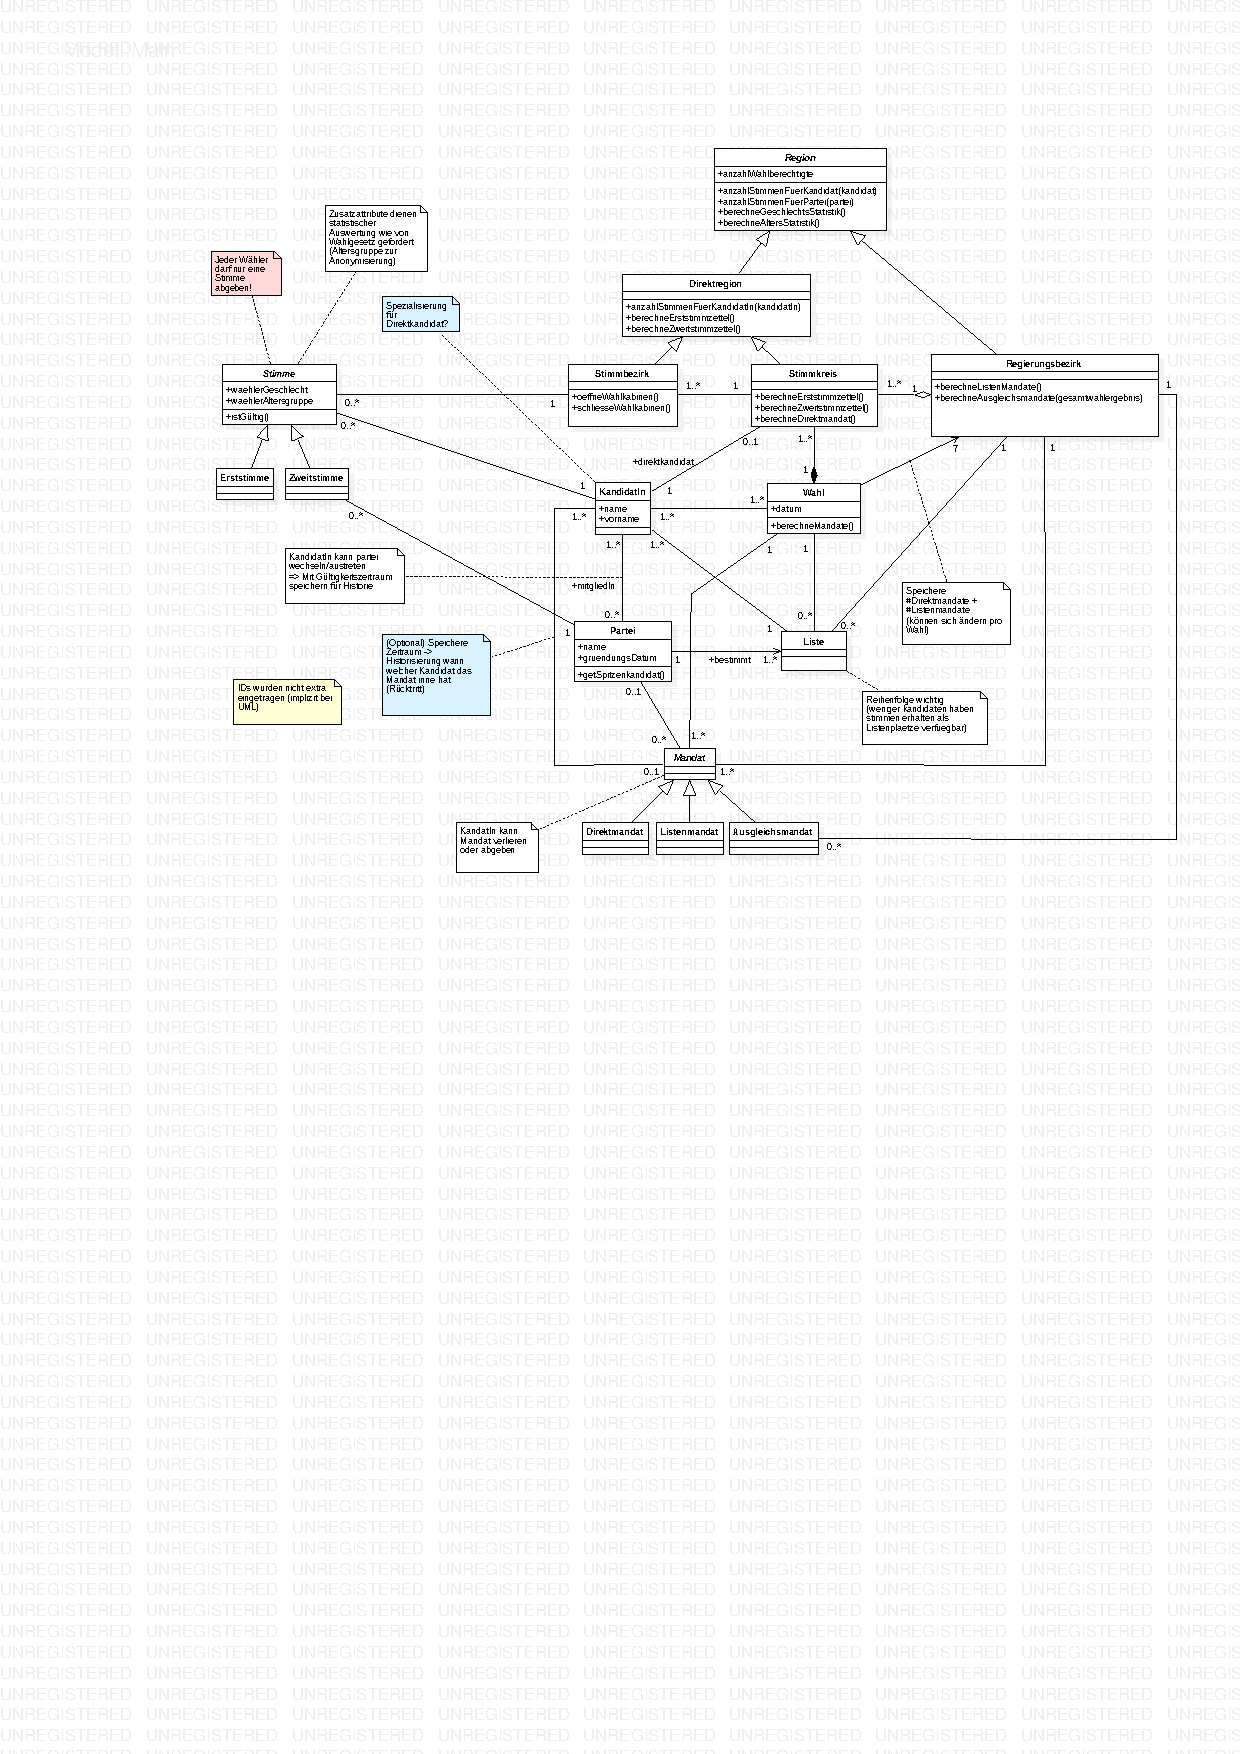
\includegraphics[width=\textwidth]{../model.pdf}
\end{center}

\section{Abnahmekriterien}
Dieser Abschnitt definiert die wichtigsten Kriterien welche zwischen dem Erzeugnis und der Abnahme stehen.
Sie leiten sich hauptsächlich aus den in diesem Dokument spezifizierten Anforderungen ab.

\begin{enumerate}
  \item Die Softwareplatform ist über eine graphisch ansprechende Weboberfläche benutzbar.
  \item Das System erlaubt die (statistische) Auswertung von realen Stimmdaten zu bayerischen Landtagswahlen, d.h. 
        insbesondere die Bestimmung der gewonnenen Mandate im Bayerischen Landtag. Dabei müssen gesetzliche
        Vorgaben genauestens eingehalten sein sowie Daten sicher, Datenschutzrechtlich korrekt und integer gehalten
        werden.
  \item Es ist möglich, gezielt die unterschiedlichen Analysen von verschiedenen Wahlvorgängen einfach zu vergleichen.
  \item WählerInnen haben durch eine bereitgestellte Oberfläche die Möglichkeit ihre Erst- und Zweitstimme abzugeben.
        Dabei muss gewährleistet sein, dass jede wahlberechtigte Person nur maximal einmal abstimmen kann, 
        Datenschutzrechtliche sowie gesetzliche Vorgaben wie das Stimmgeheimnis eingehalten werden und das System 
        insbesondere vor unbefugtem Zugriff geschützt ist.
  \item Reale Stimmdaten vergangener Wahlen können von berechtigten Nutzern, z. B. WahlleiterInnen, importiert und
        (statistisch) ausgewertet werden.
\end{enumerate}
\end{document}
